\documentclass[dvipsnames]{article}
\usepackage[english]{babel}
\usepackage{multirow}
\usepackage[letterpaper,top=2cm,bottom=2cm,left=3cm,right=3cm,marginparwidth=1.75cm]{geometry}
\usepackage{amsmath}
\usepackage{graphicx}
\usepackage{minted}
\usepackage{amsthm}
\usepackage{mathtools}
\usepackage[colorlinks=true, allcolors=blue]{hyperref}
\usepackage{fancyhdr}
\usepackage{enumerate}
\usepackage{tikz-cd}
\usepackage{mdframed}
\usepackage{multicol}

\newmintinline[java]{java}{}

\usepackage{tikz}
\usetikzlibrary{shapes}
\usetikzlibrary{arrows}

\tikzset{
  treenode/.style = {align=center, inner sep=0pt, text centered,
    font=\sffamily},
  avl_node/.style = {treenode, circle, black, draw=black,
    text width=1.5em, very thick},% arbre rouge noir, noeud rouge
  black_node/.style = {treenode, circle, white, font=\sffamily\bfseries, draw=black,
    fill=black, text width=1.5em},% arbre rouge noir, noeud noir
  red_node/.style = {treenode, circle, red, draw=red,
    text width=1.5em, very thick},% arbre rouge noir, noeud rouge
  nil_leaf/.style = {treenode, rectangle, draw=black, fill=black,
    minimum width=0.3em, minimum height=0.3em}% arbre rouge noir, nil
}

\begin{document}
\section*{Week 12. Problem set (solutions by \textcolor{blue}{Karim Khabibrakhmanov})}

\thispagestyle{fancy}
\lhead{Karim Khabibrakhmanov (\texttt{k.khabibrakhmanov@innopolis.university}), group B24-DSAI-05}

\begin{enumerate}

  \item
  
  \begin{multicols}{2}
  Run the Floyd-Warshall algorithm~\cite[\S 23.2]{Cormen2022} on the following graph.

  Consider vertices alphabetically ({\small A, B, C, D, E}).
  Show the state of distance matrix $D$ after each iteration of outer loop in the algorithm.
  Since the graph has 5 vertices, you must provide five $5 \times 5$ matrices in your answer.
  No justification is required.
  
  \columnbreak

\begin{center}
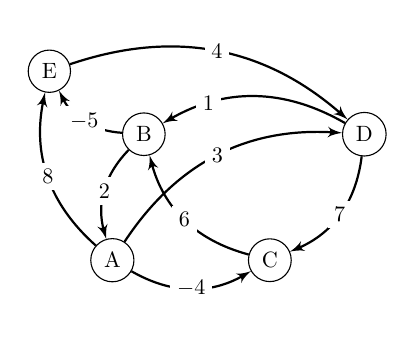
\begin{tikzpicture}[scale=0.8, every node/.style={scale=0.8}]

\tikzset{vertex/.style = {shape=circle,draw,minimum size=1.5em}}
\tikzset{edge/.style = {->,> = latex',thick}}
% vertices
\node[vertex] (a) at  (0.5,-1)   {B};
\node[vertex] (b) at  (0,-3)   {A};
\node[vertex] (c) at  (4,-1)   {D};
\node[vertex] (d) at  (-1,0)   {E};
\node[vertex] (e) at  (2.5,-3)  {C};
%edges
\draw[edge] (a) to[bend right] node {\colorbox{white}{$2$}} (b);
\draw[edge] (a) to[bend left] node {\colorbox{white}{$-5$}} (d);
\draw[edge] (b) to[bend left] node {\colorbox{white}{$3$}} (c);
\draw[edge] (b) to[bend left] node {\colorbox{white}{$8$}} (d);
\draw[edge] (b) to[bend right] node {\colorbox{white}{$-4$}} (e);
\draw[edge] (c) to[bend right, near end] node {\colorbox{white}{$1$}} (a);
\draw[edge] (c) to[bend left] node {\colorbox{white}{$7$}} (e);
\draw[edge] (d) to[bend left] node {\colorbox{white}{$4$}} (c);
\draw[edge] (e) to[bend left] node {\colorbox{white}{$6$}} (a);
\end{tikzpicture}
\end{center}
\end{multicols}%

  \color{blue}
  \textbf{Answer:}\\
  \begin{center}
    \begin{tabular}{|c|c|c|c|c|}
      \hline $0$ & $\infty$ & $-4$ & $3$ & $8$ \\
      \hline $2$ & $0$ & $\infty$ & $\infty$ & $-5$ \\
      \hline $\infty$ & $6$ & $0$ & $\infty$ & $\infty$ \\
      \hline $\infty$ & $1$ & $7$ & $0$ & $\infty$ \\
      \hline $\infty$ & $\infty$ & $\infty$ & $4$ & $0$ \\
      \hline
    \end{tabular}
    \end{center}

    \begin{center}
    \textbf{D^{(1)} = }
    \begin{tabular}{|c|c|c|c|c|}
      \hline $0$ & $\infty$ & $-4$ & $3$ & $8$ \\
      \hline $2$ & $0$ & $-2$ & $5$ & $-5$ \\
      \hline $\infty$ & $6$ & $0$ & $\infty$ & $\infty$ \\
      \hline $\infty$ & $1$ & $7$ & $0$ & $\infty$ \\
      \hline $\infty$ & $\infty$ & $\infty$ & $4$ & $0$ \\
      \hline
    \end{tabular}
    \end{center}
    
    \begin{center}
    \textbf{D^{(2)} = }
    \begin{tabular}{|c|c|c|c|c|}
      \hline $0$ & $\infty$ & $-4$ & $3$ & $8$ \\
      \hline $2$ & $0$ & $-2$ & $5$ & $-5$ \\
      \hline $8$ & $6$ & $0$ & $11$ & $1$ \\
      \hline $3$ & $1$ & $-1$ & $0$ & $-4$ \\
      \hline $\infty$ & $\infty$ & $\infty$ & $4$ & $0$ \\
      \hline
    \end{tabular}
    \end{center}

    \begin{center}
    \textbf{D^{(3)} = }
    \begin{tabular}{|c|c|c|c|c|}
      \hline $0$ & $2$ & $-4$ & $3$ & $-3$ \\
      \hline $2$ & $0$ & $-2$ & $5$ & $-5$ \\
      \hline $8$ & $6$ & $0$ & $11$ & $1$ \\
      \hline $3$ & $1$ & $-1$ & $0$ & $-4$ \\
      \hline $\infty$ & $\infty$ & $\infty$ & $4$ & $0$ \\
      \hline
    \end{tabular}
    \end{center}


    \begin{center}
    \textbf{D^{(4)} = }
    \begin{tabular}{|c|c|c|c|c|}
      \hline $0$ & $2$ & $-4$ & $3$ & $-3$ \\
      \hline $2$ & $0$ & $-2$ & $5$ & $-5$ \\
      \hline $8$ & $6$ & $0$ & $11$ & $1$ \\
      \hline $3$ & $1$ & $-1$ & $0$ & $-4$ \\
      \hline $7$ & $5$ & $3$ & $4$ & $0$ \\
      \hline
    \end{tabular}
    \end{center}

    \begin{center}
    \textbf{D^{(5)} = }
    \begin{tabular}{|c|c|c|c|c|}
      \hline $0$ & $2$ & $-4$ & $1$ & $-3$ \\
      \hline $2$ & $0$ & $-2$ & $-1$ & $-5$ \\
      \hline $8$ & $6$ & $0$ & $5$ & $1$ \\
      \hline $3$ & $1$ & $-1$ & $0$ & $-4$ \\
      \hline $7$ & $5$ & $3$ & $4$ & $0$ \\
      \hline
    \end{tabular}
    \end{center}


    
  \color{black}

  \clearpage
  \item
  
  \begin{multicols}{2}
  Run Dijkstra's algorithm~\cite[\S 22.3]{Cormen2022} on the following graph $\mathcal{G}$, starting at vertex $S$,
  and answer the questions below.

  \columnbreak
  
  \begin{center}
  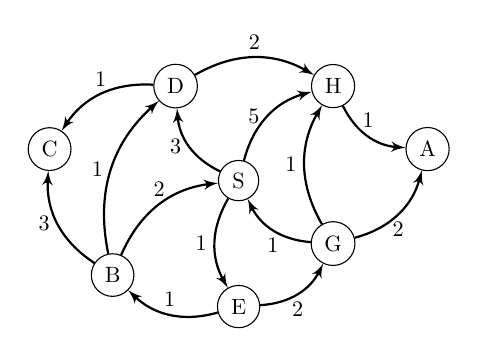
\begin{tikzpicture}[scale=0.8, every node/.style={scale=0.8}]
  
  \tikzset{vertex/.style = {shape=circle,draw,minimum size=1.5em}}
  \tikzset{edge/.style = {->,> = latex',thick}}
  % vertices
  \node[vertex] (a) at  (4,4)   {A};
  \node[vertex] (b) at  (-1,2)   {B};
  \node[vertex] (c) at  (-2,4)   {C};
  \node[vertex] (d) at  (0,5)   {D};
  \node[vertex] (e) at  (1,1.5)  {E};
  \node[vertex] (s) at  (1,3.5)  {S};
  \node[vertex] (g) at  (2.5,2.5) {G};
  \node[vertex] (h) at  (2.5,5)  {H};
  %edges
  \draw[edge] (h) to[bend right, above] node {$1$} (a);
  \draw[edge] (b) to[bend left,  left]  node {$3$} (c);
  \draw[edge] (b) to[bend left,  left] node {$1$} (d);
  \draw[edge] (d) to[bend right, above] node {$1$} (c);
  \draw[edge] (d) to[bend left,  above] node {$2$} (h);
  \draw[edge] (e) to[bend left,  above] node {$1$} (b);
  \draw[edge] (s) to[bend left,  left] node {$3$} (d);
  \draw[edge] (s) to[bend right, left] node {$1$} (e);
  \draw[edge] (e) to[bend right,  below]  node {$2$} (g);
  \draw[edge] (g) to[bend left,  below]  node {$1$} (s);
  \draw[edge] (g) to[bend left,  left] node {$1$} (h);
  \draw[edge] (g) to[bend right, below] node {$2$} (a);
  \draw[edge] (s) to[bend left,  left] node {$5$} (h);
  \draw[edge] (b) to[bend left,  above] node {$2$} (s);
  \end{tikzpicture}
  \end{center}

\end{multicols}

  \begin{enumerate}
    \item Draw a shortest paths tree of the graph $\mathcal{G}$.

    \color{blue}
    \textbf{Answer:}
    \begin{center}
      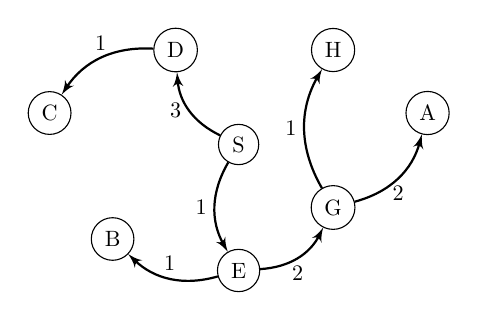
\begin{tikzpicture}[scale=0.8, every node/.style={scale=0.8}]
      
      \tikzset{vertex/.style = {shape=circle,draw,minimum size=1.5em}}
      \tikzset{edge/.style = {->,> = latex',thick}}
      % vertices
      \node[vertex] (a) at  (4,4)   {A};
      \node[vertex] (b) at  (-1,2)   {B};
      \node[vertex] (c) at  (-2,4)   {C};
      \node[vertex] (d) at  (0,5)   {D};
      \node[vertex] (e) at  (1,1.5)  {E};
      \node[vertex] (s) at  (1,3.5)  {S};
      \node[vertex] (g) at  (2.5,2.5) {G};
      \node[vertex] (h) at  (2.5,5)  {H};
      %edges
      
      \draw[edge] (g) to[bend right, below] node {$2$} (a);
      \draw[edge] (d) to[bend right, above] node {$1$} (c);
      \draw[edge] (e) to[bend left,  above] node {$1$} (b);
      \draw[edge] (s) to[bend left,  left] node {$3$} (d);
      \draw[edge] (s) to[bend right, left] node {$1$} (e);
      \draw[edge] (e) to[bend right,  below]  node {$2$} (g);
      \draw[edge] (g) to[bend left,  left] node {$1$} (h);
      
      \end{tikzpicture}
      \end{center}
    \color{black}

    \item Is the shortest paths tree for graph $\mathcal{G}$ unique?

    \color{blue}
    \textbf{Answer:} No
    \color{black}

    \item
    Assuming that the algorithm is using Binary Heap implementation~\cite[\S 6]{Cormen2022} of a priority queue,
    show the state of the priority queue after each iteration of the algorithm (i.e. after adding each new vertex to the shortest paths tree).
    The graph contains 8 vertices, which means that your solution must provide 8 states of the Binary heap.
    Each heap state must be represented as an array.

    For example, a binary min-heap containing key-value pairs $\langle 3, a\rangle, \langle 2, b\rangle, \langle 1, c\rangle, \langle 4, d\rangle$
    may be represented as follows:

    \begin{center}
    \begin{tabular}{|c|c|c|c|}
      \hline \makebox[\widthof{000}][c]{$1, c$}
          & \makebox[\widthof{000}][c]{$3, a$}
          & \makebox[\widthof{000}][c]{$2, b$}
          & \makebox[\widthof{000}][c]{$4, d$} \\
      \hline
    \end{tabular}
    \end{center}

    \color{blue}
    \textbf{Answer:}\\
    1. Add S
    \begin{tabular}{|c|c|c|c|c|}
      \hline \makebox[\widthof{000}][c]{$1,  E$}
          & \makebox[\widthof{000}][c]{$3, D$}
          & \makebox[\widthof{000}][c]{$5, H$}\\
      \hline
    \end{tabular}\\
    2. Add E
    \begin{tabular}{|c|c|c|c|c|}
      \hline \makebox[\widthof{000}][c]{$2,  B$}
          & \makebox[\widthof{000}][c]{$3, G$}
          & \makebox[\widthof{000}][c]{$3, D$}
          & \makebox[\widthof{000}][c]{$5, H$}\\
      \hline
    \end{tabular}\\
    3. Add B
    \begin{tabular}{|c|c|c|c|}
      \hline \makebox[\widthof{000}][c]{$3, G$}
          & \makebox[\widthof{000}][c]{$5, H$}
          & \makebox[\widthof{000}][c]{$3, D$}
          & \makebox[\widthof{000}][c]{$5, C$}\\
      \hline
    \end{tabular}\\
    4. Add G
    \begin{tabular}{|c|c|c|c|c|}
       \hline \makebox[\widthof{000}][c]{$3, D$}
          & \makebox[\widthof{000}][c]{$4, H$}
          & \makebox[\widthof{000}][c]{$5, C$}
          & \makebox[\widthof{000}][c]{$5, A$}\\
      \hline
    \end{tabular}\\
    5. Add D
    \begin{tabular}{|c|c|c|c|}
      \hline \makebox[\widthof{000}][c]{$4, H$}
          & \makebox[\widthof{000}][c]{$5, A$}
          & \makebox[\widthof{000}][c]{$4, C$}\\
      \hline
    \end{tabular}\\
    6. Add H
    \begin{tabular}{|c|c|c|c|}
      \hline \makebox[\widthof{000}][c]{$4, C$}
          & \makebox[\widthof{000}][c]{$5, A$}\\
      \hline
    \end{tabular}\\
    7. Add C
    \begin{tabular}{|c|c|c|c|}
      \hline \makebox[\widthof{000}][c]{$5, A$}\\
      \hline
    \end{tabular}\\
    8. Add A
    \begin{tabular}{|c|c|c|c|}
      \hline \makebox[\widthof{000}][c]{$$}\\
      \hline
    \end{tabular}\\
    \color{black}
    \color{black}
  \end{enumerate}

  \clearpage
  \item Consider a graph $\mathcal{G} = (V, E)$ that represents a computer network.
  Each edge $(u, v)$ represents a physical cable connecting two computers and
  has a \emph{length} $\ell(u, v)$ and a bandwidth $b(u, v)$.
  
  The \emph{length of a path} $P$ is computed as the sum of lengths of all edges in $P$.
  The \emph{bandwidth of a path} $P$ is computed as the minimum of bandwidth values for all edges in $P$.

  Given two paths $P_1, P_2$ in the $\mathcal{G}$ with lengths $\ell_1, \ell_2$ and bandwidth values $b_1, b_2$,
  we consider $P_1$ to be \emph{better} than $P_2$ when $\ell_1 < \ell_2$ or ($\ell_1 = \ell_2$ and $b_1 > b_2$).

  Consider a modification of Dijkstra's algorithm~\cite[\S 22.3]{Cormen2022} that finds the best paths
  in such a computer network from a single source vertex. Answer the following questions:

  \begin{enumerate}
    \item What should serve as key (priority) in the priority queue in the modified Dijkstra's algorithm?

    \color{blue}
    \textbf{Answer:} In the \textbf{Priority Queue}, the length($\ell$) should be given priority, followed by bandwidth($b$). The bandwidth($b$) takes priority when the lengths($\ell$) of two paths are equal.\\
    Key priority is lengths($\ell$).
    \color{black}

    \item Is it still possible to rely on \textsc{Decrease-Key} in the implementation?
    If yes, explain how. If no, explain why. In either case provide a brief justification (1--2 sentences).

    \color{blue}
    \textbf{Answer:} Yes

    \textbf{Justification:} \\The \textbf{Decrease-Key} function preserves strict order and monotony for a pair (length, bandwidth):
\begin{enumerate}
    \item The shorter length takes precedence
    \item With the same length, priority goes to higher bandwidth.
\end{enumerate}
    \color{black}

    \item Correctness of Dijkstra's algorithm~\cite[Theorem~22.6]{Cormen2022} has a constraint on the weight function $w$.
      What constraint on functions $\ell$ and $b$ is necessary for the correctness of the modified Dijkstra's algorithm?

    \color{blue}
    \textbf{Answer:}\\
    For the algorithm to work correctly, we need:
    \begin{enumerate}
        \item All edge lengths $\ell(u,v)$ to be non-negative ($\ell(u,v) \geq 0$)
        \item All bandwidths $b(u,v)$ to be monotonic (non-increasing along any path)
    \end{enumerate}
    

    
    \color{black}
  \end{enumerate}
\end{enumerate}

\begin{thebibliography}{BoasWrench}

\bibitem[CLRS]{Cormen2022}
Cormen, T.H., Leiserson, C.E., Rivest, R.L. and Stein, C., 2022. \emph{Introduction to algorithms, Fourth Edition}. MIT press.

\bibitem[GTG]{Goodrich2014}
M. T. Goodrich, R. Tamassia, and M. H. Goldwasser. \emph{Data Structures and Algorithms in Java.} WILEY 2014.

\end{thebibliography}

\end{document}